\newpage
\setcounter{figure}{0}

\section{Rezultati} % (fold)
\label{sec:Rezultati}

U ovom poglavlju prikazani su rezultati rada razvijenog programa za
prepozavanje statičnog znaka iz snimke prometnice vozila u pokretu.  Za
ispitivanje funkcionalnosti metode odabrana je jedna scena voženje i
jedan znak kojeg metoda treba pronaći. Znak je prikazan na
slici~\ref{fig:znak}, a scena vožnje je snimljena na osječkoj
obilaznici i prikazana na slici~\ref{fig:scena.png}.

\begin{figure}[h]
\centering
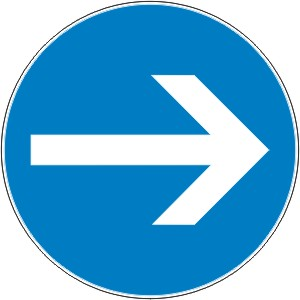
\includegraphics[scale=0.5]{figures/znak.png}
\caption{Prikaz korištenog znaka - obvezan smjer kretanja u desno}
\label{fig:znak}
\end{figure}

\begin{figure}[h]
\centering
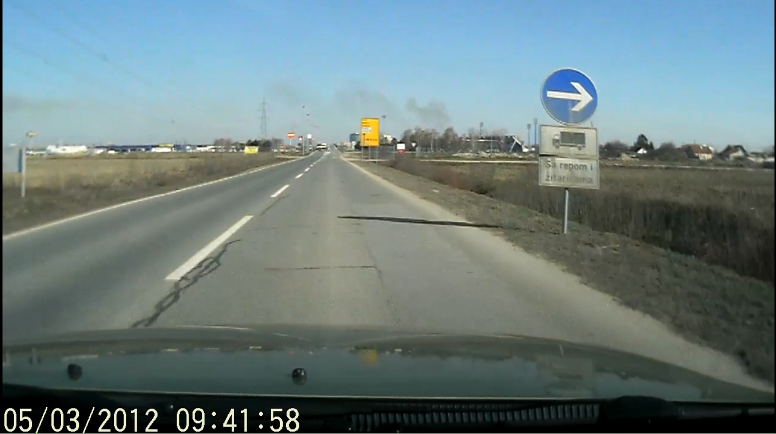
\includegraphics[scale=0.3]{figures/scena.png}
\caption{Prikaz testirane scene voznje}
\label{fig:scena.png}
\end{figure}

\newpage
\subsection{Prikaz rezultata} % (fold)
\label{sub:Prikaz rezultata}

Rezultati su prikazani na slikama s dva prozora. U prvom prozoru
prikazana je regija interesa sa scene unutar koje algoritmom usporedbe
tražimo znak. Regija interesa je odabrana na temelju pretpostavke da će
pozicija znaka bit s desne strane učitane scene. Također regija interesa
se definira kako bih se smanjila količina podataka koju algoritam mora
obraditi. U drugom prozoru prikazana je matrica rezultata koju metoda
koristi za pronalazak znaka.  Postoji nekoliko tipova rezultata:
pozitivni, negativni i lažno pozitivni. Svi tipovi rezultata su
predstavljeni dalje u tekstu. Slika~\ref{fig:01} prikazuje sličicu iz
videa sa scene na kojoj nema znaka niti ga je metoda/program našao što
je pozitivan rezultat.

\begin{figure}[h]
\centering
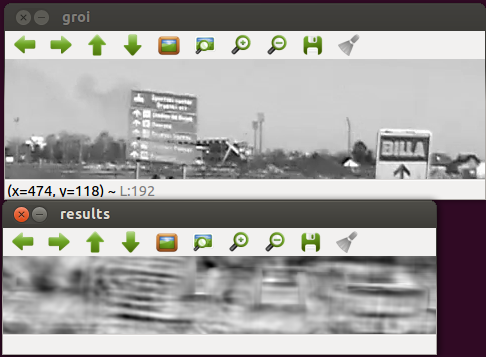
\includegraphics[scale=0.5]{figures/01.png}
\caption{Prikaz sličice videa i rezultata - pozitivan rezultat}
\label{fig:01}
\end{figure}

Lažno pozitivni rezultat prikazuje slika~\ref{fig:02} na kojoj je metoda
pronašala znak gdje nije trebala. Takvi rezultati su očekivani ali nisu
poželjni te ih se pokušalo smanjiti na što manji broj metodom opisanom 
u podpoglavlju~\ref{ssub:Eliminacija lažno pozitivnih rezultata}

\begin{figure}[h]
\centering
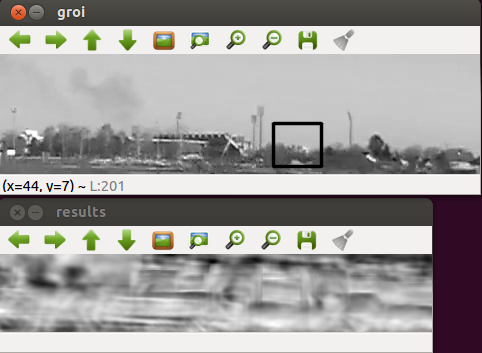
\includegraphics[scale=0.5]{figures/02.png}
\caption{Prikaz sličice videa i matrice rezultata - lažno pozitivan
rezultat}
\label{fig:02}
\end{figure}

\newpage
\begin{figure}[h]
\centering
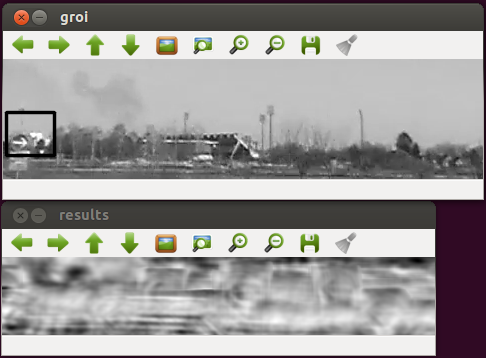
\includegraphics[scale=0.5]{figures/03.png}
\caption{Prikaz sličice videa i matrice rezultata - pozitivan rezultat }
\label{fig:03.png}
\end{figure}

Na slikama~\ref{fig:03.png} i \ref{fig:04.png}  vidi se
da je metoda uspješno pronašla znak na različitim udaljenostima odnosno
veličinama znaka iako se koristila samo jedna veličina znaka za
pronalazak. Metoda odnosno program bi se mogao unaprijediti tako da se
ugradi uspoređivanje s različitim veličinama predloška odnosno znaka.

\begin{figure}[!htb]
\minipage{0.5\textwidth}
    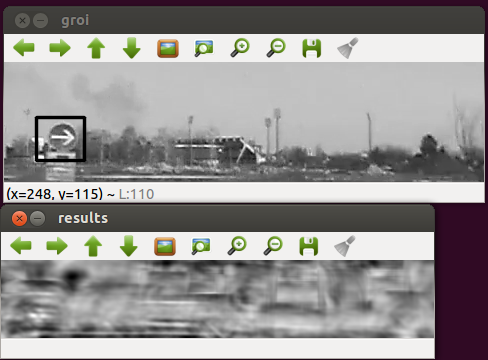
\includegraphics[width=\linewidth]{figures/04.png}
\endminipage\hfill
\minipage{0.5\textwidth}
    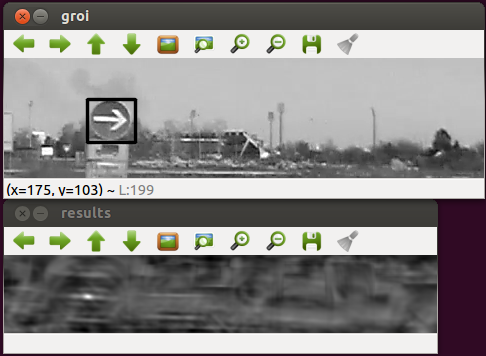
\includegraphics[width=\linewidth]{figures/05.png}
\endminipage\hfill
\caption{Prikaz sličice videa i matrice rezultata - pozitivan rezultat}
\label{fig:04.png}
\end{figure}

Matematička metoda korištena u algoritmu prikazuje pozitivne rezultate
bijelom bojom te se na slici~\ref{fig:04.png} jasno mogu vidjeti
"žarišta" u matrici rezultata.

\newpage

Slika~\ref{fig:06.png} također prikazuje uspješan pronalazak znaka kada
je i znak na izvornoj slici nešto veći nego na slici predloška.
Slika~\ref{fig:07.png} prikazuje negativan rezultat iako se na slici s
rezultatima može vidjeti "žarište" na lokaciji gdje je znak. Program se
može unaprijediti da prati relativne vrijednosti u matrici rezultata i
na taj način bi se takvi negativni rezultati mogli smanjiti.

\begin{figure}[h]
\centering
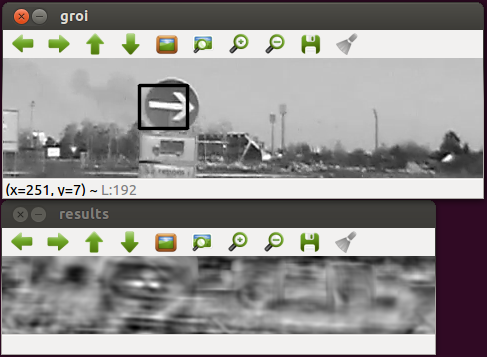
\includegraphics[scale=0.5]{figures/06.png}
\caption{Prikaz sličice videa i matrice rezultata - pozitivan rezultat}
\label{fig:06.png}
\end{figure}

\begin{figure}[h]
\centering
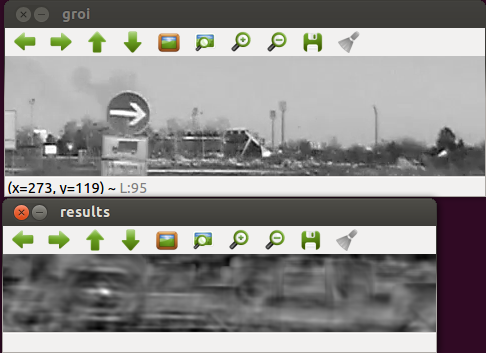
\includegraphics[scale=0.5]{figures/07.png}
\caption{Prikaz sličice videa i matrice rezultata - negativan rezultat}
\label{fig:07.png}
\end{figure}


% subsection Prikaz rezultata (end)
% section Rezultati (end)
